%!TEX root = ../thesis.tex

\chapter{Isogeometric enhanced SBFEM in 3D}
\section{Introduction}
\paragraph{}
This chapter starts with a mesh generated by the help of the octree based algorithm using STL file directly \citep{Liu2017}.
In this algorithm, the intersection is calculated between the edge of the element and the triangular surface which is an approximation of the exact geometry.
In order to achieve the geometric precision, a point projection method for 3D NURBS surface is presented.
It's computational efficiency is significantly improved by implementing a NURBS surface splitting and by utilizing the strong convex hull property of the NURBS.
The quick hull algorithm is also introduced to construct the convex hull from the control points in 3D.
Alternative method to retain the exact geometry is targeted as well.
The calculation of the intersection in \cite{Liu2017} is replaced by finding that between the edge of the element and the NURBS surface directly.

\paragraph{}
The advantage of the proposed method is that the exact geometry can be retained and hence improves the accuracy of the result.

\paragraph{}
This chapter will be organized as followed:
points projection of the NURBS surface is introduced at the beginning, together with the surface splitting and the convex hull construction.
After that, the calculation of the straight line with the NURBS surface is developed.
Furthermore, a brief introduction on SBFEM formulation in 3D elasticity is presented.
The accuracy and the convergence properties of the proposed method are demonstrated with benchmark problems in the context of linear elasticity.
Some other mesh examples from complex geometric input are also plotted at the end of this chapter.

\section{Points projection on NURBS surface}
\textcolor{red}{
\subsection{Surfaces division}
\label{oct_sc:surface_division}
\paragraph{}
Mapping points back to NURBS surfaces in 3D can be extremely time consuming as there is no known close form mathematical solution.
Every point takes about ten to hundreds iterations before it can find the nearest projection point on the NURBS surface, depending on the size of the projection surface.
However, in the problem that the proposed method is targeting, reasonably complex geometry will be expected.
As a result, points projection back to such kind of NURBS surfaces may takes much more computational time than any others do and it may be necessary to find a more complicated but computational efficient algorithm other than the naive implementation.

\paragraph{}
One concept that can be utilized to improve the efficiency here is the ``divided and conquer''.
As the time complexity of the naive algorithm is $O(n^3)$ where $n$ is directly correlated to the order and the number of control points used to describe the NURBS surfaces, dividing a surface into two generally will make the projection algorithm four times faster than it is before.
Consequently, breaking the origin NURBS surfaces into as many as it can could be a one of the practical practices.

\paragraph{}
Surfaces division can be performed by the help of knot insertion (\ref{lr_sec:nurbs_knot_ins}).
Assuming a NURBS surface defined by two knot vectors\\
$
V_1 = [-1, -1, -1, a_1, a_2, \dots, a_n , 1, 1, 1]
$\\
and
$
V_2 = [-1, -1, -1, b_1, b_2, \dots, b_m, 1, 1, 1]
$.\\
Several knots will be inserted into these two vector so that all interior knots will repeated $p+1$ times and $p$ stands for the order of the NURBS surface in that direction.
After knot insertion, the same NURBS surface will now be described by two new vectors\\
$
V_1^\prime = [-1, -1, -1, a_1, a_1, a_1, a_2, a_2, a_2, \dots, a_n , 1, 1, 1]
$\\
and
$
V_2^\prime = [-1, -1, -1, b_1, b_1, b_1, b_2, b_2, b_2, \dots, b_m, 1, 1, 1]
$.\\
Extraction then can be conducted by take the sub-matrix from the generated control points matrix $P^\prime$ and weight matrix $w^\prime$.

\paragraph{}
Fig.~\ref{oct_fig:nurbs_division} shows a sub-division of breaking a cylinder surface into four smaller ones.

\begin{figure}[h!]
    \centering
    \begin{subfigure}[b]{0.4\linewidth}
        \centering
        \scalebox{0.27}{
            
\includegraphics{octree/images/NURBSParent.png}
        }
        \caption{Original NURBS surface}
    \end{subfigure}
    \begin{subfigure}[b]{0.4\linewidth}
        \centering
        \scalebox{0.25}{
            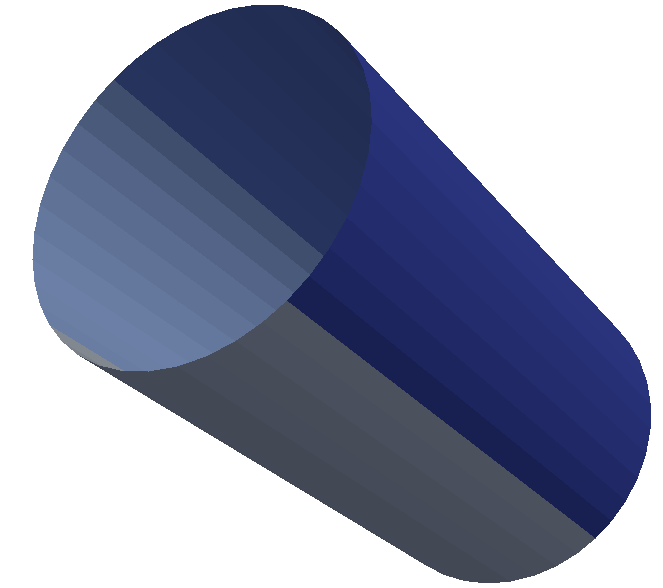
\includegraphics{octree/images/NURBSChildren.png}
        }
        \caption{Subdivided child NURBS surfaces}
    \end{subfigure}
    \caption{NURBS surface subdivision}
    \label{oct_fig:nurbs_division}
\end{figure}

\subsection{Matrix Representation for Rational Bezier Surface} 
\paragraph{}
A tensor-product rational Bézier surface of degree $(p_1,p_2)$ can be expressed as
\begin{equation*}
	\phi(u,v)\in\mathbf{R}^2 \rightarrow \frac{\sum_{i=0}^{p_1}\sum_{j=0}^{p_2}w_{i,j}\mathbf{P}_{i,j}B_i^{p_1}(t)B_j^{p_2}(t) }{\sum_{i=0}^{p_1}\sum_{j=0}^{p_2}w_{i,j}B_i^{p_1}(t)B_j^{p_2}(t)}
\end{equation*}
For the surface, $\mathbf{L}$ and $\mathbf{R}$ with order $(v_1,v_2)$
\begin{equation*}
	\mathbf{L} =
	\begin{bmatrix}
		B_0^{v_1+p_1}(u)B_0^{v_2+p_2}(v) & B_1^{v_1+p_1}(u)B_0^{v_2+p_2}(v) & \dots & B_{v_1+p_1}^{v_1+p_1}(u)B_{v_2+p_2}^{v_2+p_2}(v)
	\end{bmatrix}
\end{equation*}
\begin{equation*}
	\mathbf{R} =
	\begin{bmatrix}
		B_0^{v_1}(u)B_0^{v_2}(v)f_0(u,v) & B_0^{v_1}(u)B_1^{v_2}(v)f_0(u,v) & \dots & B_{v_1}^{v_1}(u)B_{v_2}^{v_2}(v)f_3(u,v)
	\end{bmatrix}
\end{equation*}
Following the same manner in the previous section, it can be derived that 
\begin{equation}
	\mathbf{S}_{\left( (i+k)(v_2+p_2+1)+j+l, l(v1+1)+k\right)} = 
	\frac{\mathbf{C}_k^{v_1}\mathbf{C}_l^{v_2}\mathbf{C}_i^{p_1}\mathbf{C}_j^{p_2}} 
		{\mathbf{C}_{i+k}^{v_1+d_2}\mathbf{C}_{j+l}^{v_2+d_2}}c_{(i,j)}
\end{equation}

\subsection{Property of $\mathbf{M_v}$ Matrix}
As described in the previous sections, the $\mathbf{M_v}$ matrix is defined so that
\begin{equation*}
	\begin{bmatrix}
	\psi_1(t_0) \dots \psi_{m_v}(t_0)
	\end{bmatrix}
	\times
	\mathbf{M_v(\mathbf{P})}
	= \vec{0}
\end{equation*}
where $\mathbf{P}$ is a point on the rational bezier curve/surface.
The order $v$ shall be no less than a critical value and it is proofed to be
\begin{itemize}
	\item $v>max(p-1,1)$ for rational bezier curve
	\item $(v_1,v_2) > (2p_1 -1, p_2 -1)$ or  $(v_1,v_2) > (p_1 -1, 2p_2 -1)$
\end{itemize}
The following properties are proofed in \cite{Laurent2014}
\begin{enumerate}
	\item For all degrees $geq$ critical degree and all point $\in\mathbf{R}^3$ , rank($\mathbf{M_v}(\mathbf{P})$) $<m_v$ if and only if $\mathbf{P}\in$ the closure of $\overline{Im}(\phi)$.
	\item If $\mathbf{P}\in\mathbf{R}^3$ is a point with a unique pre-image by $\phi$, the dimension of the null space of $\mathbf{M_v}(\mathbf{P})^T$ is one. 
	\item $\delta\mathbf{M_v}(\mathbf{P}) = 0$ if $\mathbf{P} \in\overline{Im}(\phi)$
\end{enumerate}
where 
\begin{equation*}
	\delta\mathbf{M_v}(\mathbf{P}) = \prod_{i=1}^{m_v}\sigma_i(\mathbf{M_v}(\mathbf{P}))
\end{equation*}
and $\sigma_i$ is the diagonal of $\Sigma$ in the SVD decomposition of $\mathbf{M_v}(\mathbf{P})=U\Sigma V^T$

\begin{enumerate}
	\setcounter{enumi}{3}
	\item $\forall\mathbf{P}\in\mathbf{R}^3$, $d(\mathbf{P},\overline{Im}(\phi))^{n_1}\leq c_1 \delta\mathbf{M_v}(\mathbf{P})$
	\item $\forall\mathbf{P}\in\mathbf{R}^3$, $\delta\mathbf{M_v}(\mathbf{P})^{n_2}\leq c_2 d(\mathbf{P},\overline{Im}(\phi))^{n_2} $
\end{enumerate}
where $c_1,c_2,n_1,n_2$ are constant.\\
These two properties give a distance function like function of the $M_v$ matrix. When the point get away to the surface, $\delta\mathbf{M_v}$ is getting larger and vice versa.vise visa.
\paragraph{}
If the point is on the curve/surface, in which case $\delta\mathbf{M_v}(\mathbf{P}) = 0$, the corresponding parameter value on the curve/surface can be easily found by a SVD numerically.\\
The computation of the null space of $\mathbf{M_v}(\mathbf{P}) $ will give a single vector $V=[v_1,v_2,\dots,v_{m_v}]$based on 2 and $V$ will be proportional to 
\begin{equation*}
	\begin{bmatrix}
	\psi_1(t_0) \dots \psi_{m_v}(t_0)
	\end{bmatrix}
\end{equation*}
More specifically, it will be proportional to
\begin{equation*}
	\begin{bmatrix}
		B_0^v & B_1^v & \dots
	\end{bmatrix}
\end{equation*}
for the rational bézier curves and
\begin{equation*}
	\begin{bmatrix}
		B_0^{v1}B_0^{v2} & B_0^{v1}B_1^{v2} & \dots
	\end{bmatrix}
\end{equation*}
for the rational bézier surfaces.
}


\section{Introduction of SBFEM in 3D}

\section{Numerical examples}
\section{Pressurized hollow sphere}
\paragraph{}
The problem is a pressurized hollow sphere subjected to internal pressure. The geometry of the problem is described in fig.\ref{oct_fig:ex_pre-hollow-sphere}. 

\begin{figure}[h!]
  \centering
  \scalebox{1}{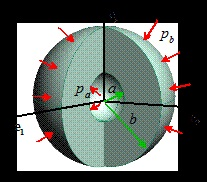
\includegraphics{octree/ex_images/oct_ex_image021.jpg}}
  \caption{Pressurized hollow sphere}
  \label{oct_fig:ex_pre-hollow-sphere}
\end{figure}

\paragraph{}
In the example, the external pressure is set to be zero so that only the internal one is considered. $a=20, b=150, p_a = 10,p_b = 0, E=200,\nu=0.3$. Instead of a quarter of a hollow sphere, a cubic with a spherical hole is analysed. Displacement boundary condition is applied on all of the boundary surface. First order tetrahedral element is adopted to calculated the displacement and stress and compared to the exact solution as in eq.~\ref{oct_eq:ex_hollow_sphere_ana_sol} in spherical coordinate.

\begin{subequations}
\begin{align}
  u & = \frac{1}{2E(b^3-a^3)R^2}\left\{ 2(p_aa^3-p_bb^3)(1-2\nu)R^3+(p_a-p_b)(1+\nu)b^3a^3\right\}\\
  \sigma_{RR} & = \frac{p_aa^3-p_bb^3}{b^3-a^3} - \frac{(p_a-p_b)b^3a^3}{(b^3-a^3)R^3}\\
  \sigma_{\theta\theta} & = \frac{p_aa^3-p_bb^3}{b^3-a^3} + \frac{(p_a-p_b)b^3a^3}{2(b^3-a^3)R^3}\\
  \sigma_{\phi\phi} & = \sigma{\theta\theta}
  \label{oct_eq:ex_hollow_sphere_ana_sol}
\end{align}
\end{subequations}

\paragraph{}
The tensor transformation from spherical coordinate to cartesian coordinate can be written as eq.\~ref{eqn:transformation} with according to fig.~\ref{octree_fig:oct_ex_hollow_sphere_tran}.
\begin{subequations}
  \begin{align}
    \begin{bmatrix}
      S_{xx} & S_{xy} & S_{xz} \\
      S_{xy} & S_{yy} & S_{yz} \\
      S_{xz} & S_{yz} & S_{zz} \\
    \end{bmatrix} = T\begin{bmatrix}
      S_{RR} & S_{R\theta} & S_{R\phi} \\
      S_{R\theta} & S_{\theta\theta} & S_{\theta\phi}\\
      S_{R\phi} & S_{\theta\phi} & S_{\phi\phi} \\
    \end{bmatrix} T^T\\
  T = 
\begin{bmatrix}
\sin\theta\cos\phi & \cos\theta\cos\phi & -\sin\phi \\
\sin\theta\sin\phi & \cos\theta\sin\phi & \cos\phi  \\
\cos\theta & -\sin\theta & 0 \\
\end{bmatrix}
\end{align}
\label{eqn:transformation}
\end{subequations}

\begin{figure}[h!]
    \centering
    \scalebox{1}{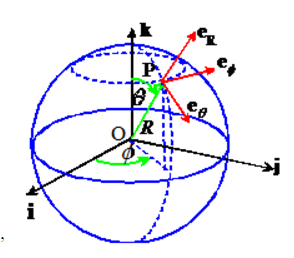
\includegraphics{octree/ex_images/oct_ex_tran.png}}
    \caption{Coordinate transformation}
    \label{octree_fig:oct_ex_hollow_sphere_tran}
  \end{figure}
  
\paragraph{}
In the example, $a = 10,b = 50, E=20,\nu = 0.2,P_a = 10$. For simplification, only a quarter of the sphere is analysed as shown in fig.~\ref{oct_fig:ex_hollow_sphere_meshP}

\begin{figure}[h!]
  \centering
  \scalebox{0.5}{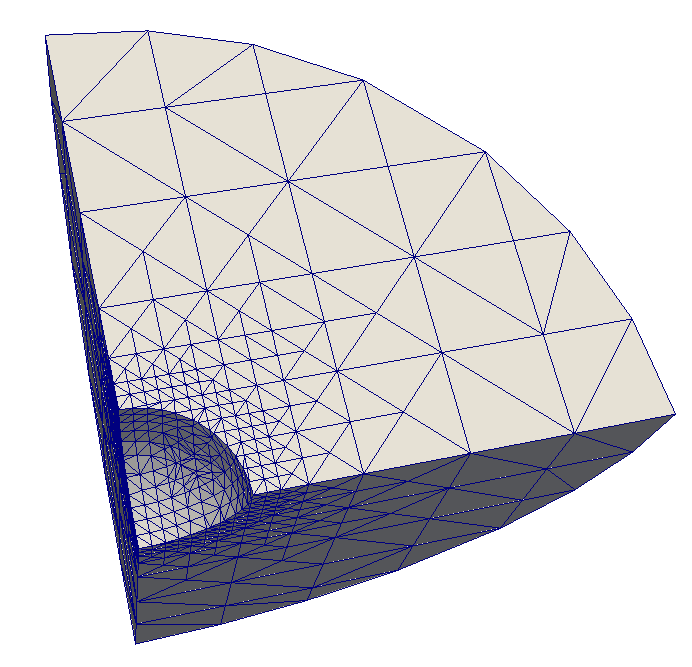
\includegraphics{octree/ex_images/oct_ex_mesh.png}}
  \caption{Mesh of the problem}
  \label{oct_fig:ex_hollow_sphere_meshP}
\end{figure}

Stress boundary in Eq.~\ref{oct_eq:ex_sphere_hole_bond_str} condition is applied on two spherical surfaces.
\begin{subequations}
    \begin{align}
    \sigma_{RR}(R=a,\phi,\theta) & = \frac{p_aa^3-p_bb^3}{b^3-a^3} - \frac{(p_a-p_b)b^3a^3}{(b^3-a^3)R^3}\\
    u_z(x,y,0) &= 0\\
    u_y(x,0,z) & = 0 \\
    u_x(0,y,z) & = 0
  \end{align}
\label{oct_eq:ex_sphere_hole_bond_str}
\end{subequations}

The convergence study is plotted in Fig.~\ref{oct_fig:ex_hollow_sphere_conv}
\begin{figure}[h!]
    \centering
    \scalebox{0.5}{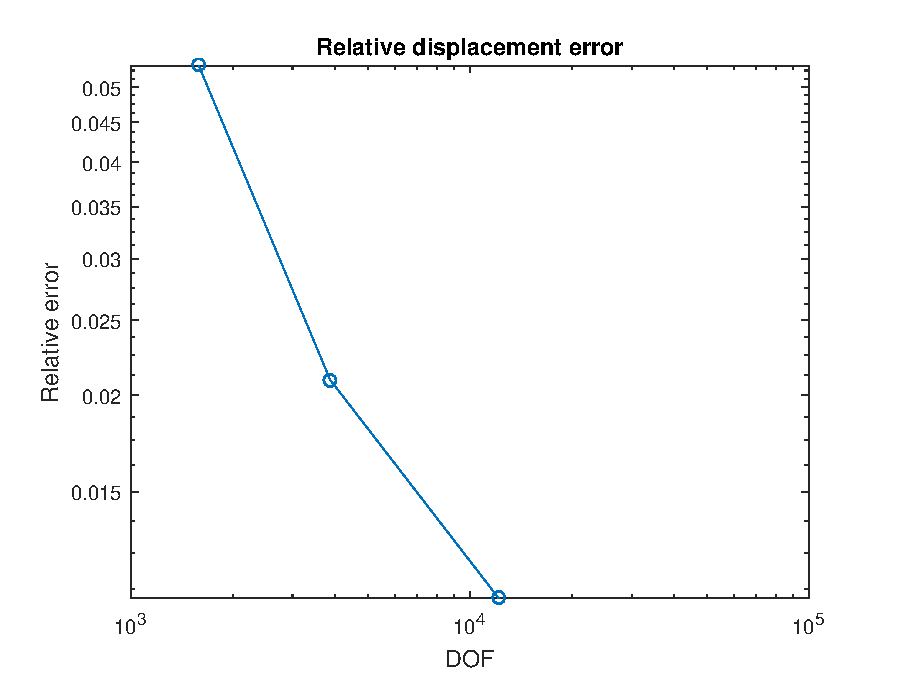
\includegraphics{octree/ex_images/ex_sphere_hole_conv.eps}}
    \caption{Convergence of displacement error}
    \label{oct_fig:ex_hollow_sphere_conv}
  \end{figure}
\subsection{Capsule Cutting From the Cuboid with Bending}
\paragraph{}
The example is a capsule section cutting from a cuboid with pure bending illustrated in Fig.~\ref{oct_fig:ex_caplus_layout} and the generated mesh is plotted in Fig.~\ref{oct_fig:ex_caplus_mesh1.png}.
\begin{figure}[h!]
  \centering
  \scalebox{.5}{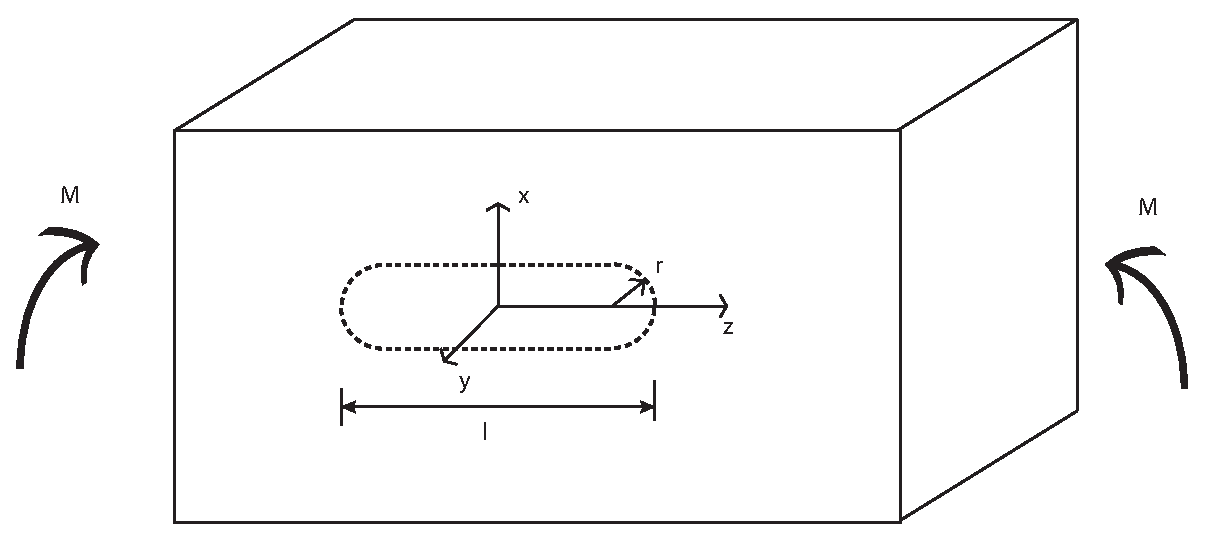
\includegraphics{octree/ex_images/oct_ex_caplus_rect.eps}}
  \caption{Problem layout}
  \label{oct_fig:ex_caplus_layout}
\end{figure}
%
\begin{figure}[h!]
  \centering
  \scalebox{.3}{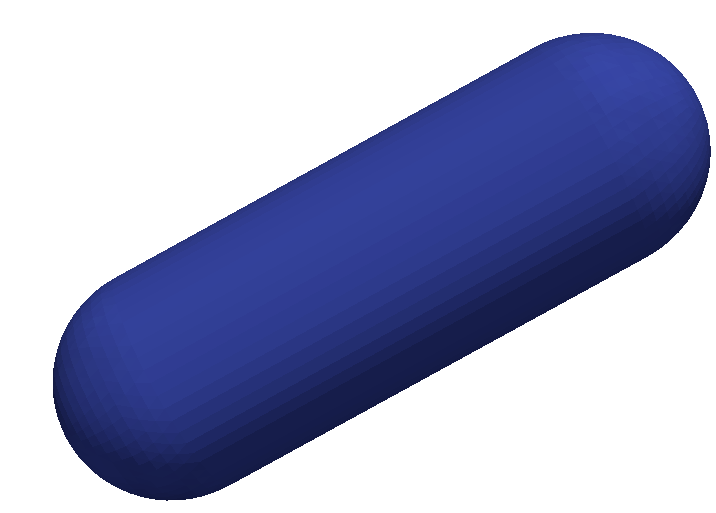
\includegraphics{octree/ex_images/oct_ex_caplus_geo.png}}
  \caption{Geometry of the capsule}
  \label{oct_fig:ex_caplus_geo}
\end{figure}
%
\begin{figure}[h!]
    \centering
    \begin{subfigure}[b]{1\linewidth}
        \centering
        \scalebox{.3}{
            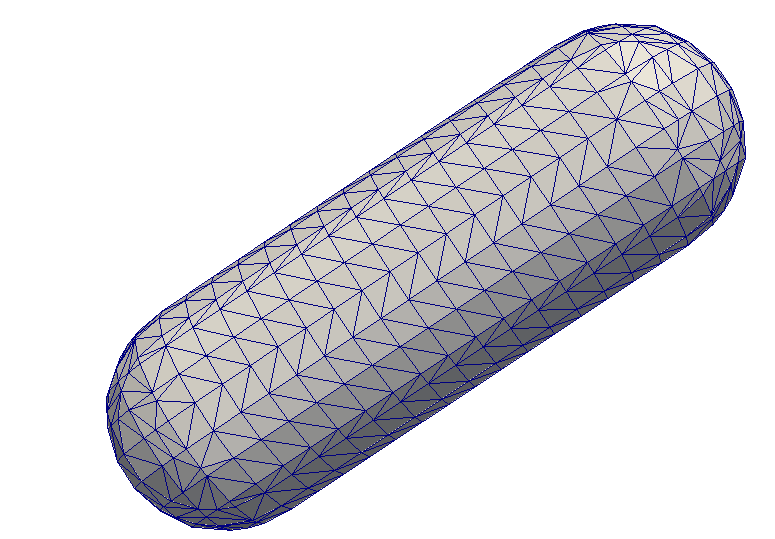
\includegraphics{octree/ex_images/oct_ex_caplus_mesh1.png}
        }
    \end{subfigure}
    \begin{subfigure}[b]{1\linewidth}
        \centering
        \scalebox{.3}{
            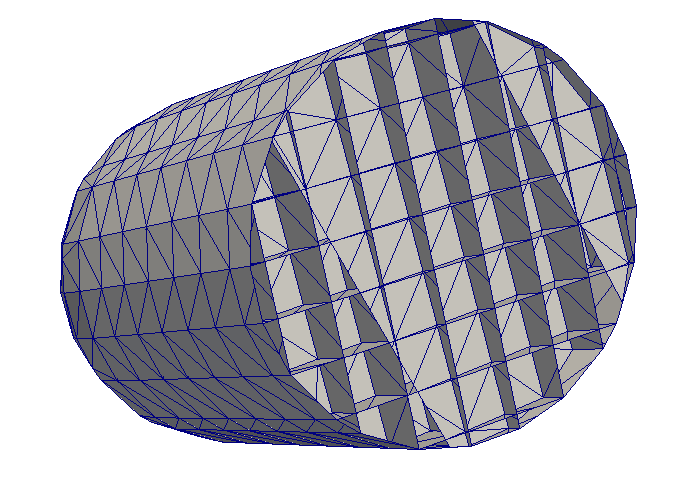
\includegraphics{octree/ex_images/oct_ex_caplus_mesh2.png}
        }
    \end{subfigure}
    \caption{Mesh of the Capsule}
    \label{oct_fig:ex_caplus_mesh1.png}
\end{figure}
%
The displacement analytical solution \citep{Tim1951} is applied on the outer surface of the capsule as the boundary condition and the displacement and \hl{the} stress (Eq.~\ref{eqn:caplus_stress}) inside is compared to the analytical solution.
All stress component \hl{except} $\sigma_z$ is zero.

\begin{subequations}
\begin{align}
  u_x &= -\frac{1}{2R}\left[z^2 + \nu \left(x^2 - y^2 \right)\right]\\
  u_y &= -\frac{\nu xy}{R}\\
  u_z &= \frac{xz}{R} 
  \label{eqn:capluse_displacement}
\end{align}
\end{subequations}

\begin{equation}
  \sigma_x = \frac{Ex}{R}
  \label{eqn:caplus_stress}
\end{equation}
%
In the numerical calculation, The dimension of the outer cuboid will not affect the result because of the independence of the analytical solution (Eq.\ref{eqn:capluse_displacement}).
6-nodes triangular element\hl{s are} used to achieve an exact solution.
The geometric properties are: $l=\SI{100}{\meter}$ and $r=\SI{17.5}{\meter}$
The material properties are: $\nu=0.2$ and $E=\SI{30}{\newton \per \square \meter}$.
The error of the displacement is calculated as followed.
\begin{subequations}
\begin{align}
e_u &= \frac{||u_{ex} - u||}{||u_{ex}||}\\
e_s &= \frac{||\sigma_{ex} - \sigma||}{||\sigma_{ex}||}
\end{align}
\end{subequations}
%
The error of the displacement norm is $1.7563\times 10^{-14}$ and the error of the stress norm is $1.3184\times 10^{-9}$.


\section{Conclusions}